\pagebreak
\subsection{Software Design}
\subsubsection{Purpose}
The purpose of the software is to automate control of the valves so that they will be opened/closed at the target altitude. Moreover, the software will store housekeeping data from sensors, pump, and valves states to the on-board memory storage device. Logging sensor data is necessary in order to determine a vertical profile of the analyzed samples:

\begin{quote}
In order to determine the vertical profiles of CO$_2$, CH$_4$, and CO from the analysis of sampled air, measurements of several atmospheric parameters are needed [...]. The two most important parameters are the ambient pressure and the mean coil temperature. These parameters will be recorded by the AirCore-HR (High Resolution) electronic data package. Mean coil temperature is obtained by taking the mean of three temperatures recorded by independent probes located at different positions along the AirCore-HR.\cite{Membrive}
\end{quote}

Both the ambient pressure and the sampling container temperature are also essential for AAC sampling bags. The temperature data will be collected by the sensors near the sampling bags.

The software shall also transmit data to the ground so that the team can monitor the conditions of the experiment in real time. Telecommand is also needed to overwrite pre-programmed sampling scheduled in case of automation failure or to mitigate unexpected changes in the flight path and reached altitudes. It will also be used to test the system, especially valves and heaters.\par
\subsubsection{Design} \label{sec:4.8.2}
\begin{enumerate}[label=(\alph*)]
\item{Process Overview}\\
The software which run on the Arduino reads from the sensors through the analog, I2C, and SPI interfaces. The sensors provides temperature, pressure, airflow, and humidity data. The acquired data will be time-stamped and stored in the on-board SD card and transmitted via the E-Link System to the ground station. Then according to the pressure/altitude, the software controls the valves which will allow the air to flow inside the tube and bags. Figure \ref{processOverview} visually explain the process flow.

\begin{figure}[H]
    \centering
    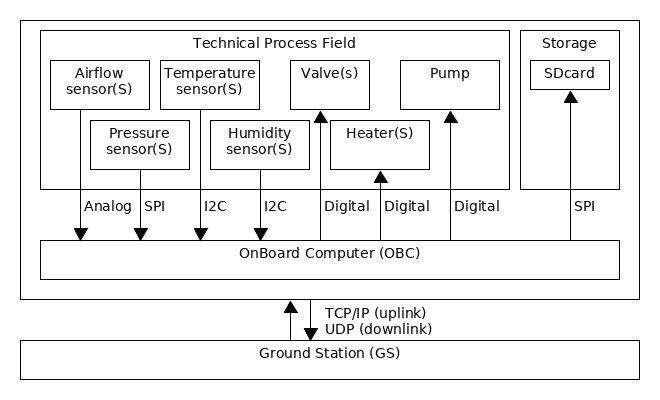
\includegraphics[width=0.85\textwidth]{4-experiment-design/img/Process-overview-V0-2.png}
    \caption{The Process Overview of the Experiment.}
    \label{processOverview}
\end{figure}

\item{General and Safety related concepts}\\
The watchdog timer, which is an electronic countdown timer that causes an interrupt when it reaches 0, will be used to avoid failure because of a freezing problem in the software. During normal operations, the software will set flags when done with their task. When all the flags have been set the watchdog gets reset. If any task fails to set the their flag before the watchdog elapses, the system resets, or \enquote{timing out}. Telecommands will also be used as backup in case the automation fails or otherwise become unresponsive. Telemetry will be utilized to transmit housekeeping data and the state of the valves to get confirmation of operation. Rigorous testing will be performed during the development of the project and before the launch phase to insure that that the software is capable to control the experiment.
\item{Interfaces}\\
Table \ref{tab:comIntpro} demonstrates how the components will interact with the onboard computer (OBC). Components that use SPI, will share MISO, MOSI, and CLK pins on the Arduino board. Each of them will also be connected to general pins input output (GPIO) for slave select. Furthermore, components using I2C protocol, will share Serial Data pin (SDA) and Serial Clock pin (SCL).

\begin{table}[H]
\centering
\begin{tabular}{lll}
Components interacting & Communication protocol & Interface                 \\ \hline
Pressure Sensors-OBC   & SPI                    & Arduino SPI and Digital Pins \\
Temperature sensors-OBC        & I2C                    & Arduino I2C \\
Airflow sensor-OBC     & I2C                    & Arduino I2C \\
Heaters-OBC            & Digital                & GPIO pins \\
Air pump-OBC           & Digital                & GPIO pins \\
Valve-OBC              & Digital                & GPIO pins                 \\
OBC-microSD Storage    & SPI                    & Arduino Ethernet shield   \\
OBC - E-Link           & Ethernet               & Ethernet port            
\end{tabular}%Tabular dude
\caption{Communication and interface protocols}
\label{tab:comIntpro}
\end{table}

Every transmission to/from the ground will utilize the E-link connection. The data packet which will be used is Ethernet Packet with a header contains the address of destination, followed by the data, and at the end there is a frame check sequence (FCS). The up-linked data packet will have the same structure, with header followed by commands and ended with FCS.\\
\\
The protocol that has been chosen are UDP for telemetry and TCP for telecommand. The UDP is used to prevent software getting stuck waiting for handshake from the ground if the connection is temporarily lost.\\
\\
The telecommand contain the following services:
\begin{itemize}
    \item Changing instrument modes
    \item Manually control valves, pump, and heaters
\end{itemize}

Furthermore, telemetry contain the services below:
\begin{itemize}
    \item Data from temperature, pressure, humidity, and airflow sensor
    \item Current instrument modes
    \item Instrument housekeeping data (valve, pump, and heater states)
\end{itemize}
\item{Data Acquisition and Storage}\\
Data will be stored on the SD memory card on the Arduino Ethernet Shield using the FAT16 and FAT32 filesystems. To minimize the data loss in the event of an reset we will only write to the same file in an set amount of time before closing it and open a new file. It is estimated that for the entire flight, all the sensors will produce $4.896$ MB of data. The sampling rate will be fixed at 2 sampling per second.\\
\\
The data will be collected and presented as a matrix, where the first column is the time frame, the following columns are the sensors data. After the sensors data, there will also be housekeeping data, that keeps track of the valves, and heaters states. However, the size of the housekeeping data is not expected to surpass 20 bits per sampling.\\
\\
Data will be continuously down-linked two times per second and the total telemetry size is $7.128$ MB for 10 hours of flight. On the other hand, the telecommand size will vary based on how many subcommand is sent each time. If all of the subcommand are enabled, the total size is 128 bytes. Considering the telecommand will not be sent more than once per second, the telecommand data rate is 126 bytes/sec.
\item{Process Flow}\\
The process flow can be explained with the mode diagram in Figure \ref{fig:modediag}. The software will start with Standby Mode, in which the software will get samples from all sensors. The on-board memory card contains the default sampling schedule parameters (when the sampling will start and stop), which will be read by the software in Standby Mode. This will allow users to change the sampling schedule without changing the internal code. When the software receives decreasing pressure changes readings, it will change to Normal - Ascent mode, where the software will trigger emptying of the CAC's tube by opening the valves. Then, at certain altitudes, air sampling will be conducted during Ascent Phase. During Float Phase, no sampling will be conducted. The software will go to Normal - Descent mode when it detects the increment of pressure is considerably big at which point the software will sample the air by opening the valves for each bag in their designated altitude. Considering that the gondola might not have smooth ascending/descending, the mode changes will only happen if the changes exceed certain threshold. Currently, $\SI{-20}{\pascal}$ and $\SI{20}{\pascal}$ are considered and might be changed depends on further analysis and testing. The experiment goes to SAFE mode approximately 500 m before the landing, and triggers all the valves to be closed. The Manual mode is entered with a telecommand and one for leaving it. When entering the manual mode the groundstation automatically retransmits the signal for manual mode at a set interval. If the signal is not received by the OBC within a certain amount of time it leaves manual mode and enters into standby mode.

\begin{figure}[H]
    \begin{align*}
        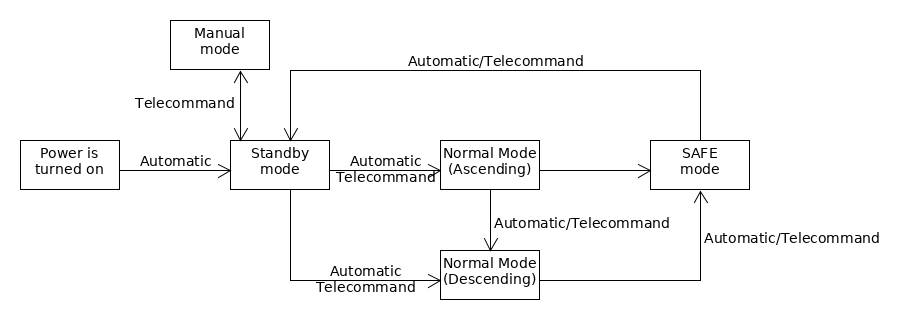
\includegraphics[width=1\linewidth]{4-experiment-design/img/state-diagram-V1-2.png}
    \end{align*}
    \caption{Process Diagram for the Modes.}\label{fig:modediag}
\end{figure}

In the sampling algorithm, it is necessary to keep track of the time because the bag cannot be filled fully (it might burst). A simple library is used to keep track of the time from the start of the experiment.\par 
At the ground station the data is stored sequentially making it possible to order the received data even without a time stamp.
\item{Modularization and Pseudo Code}\\
\begin{figure}[H]
    \begin{align*}
        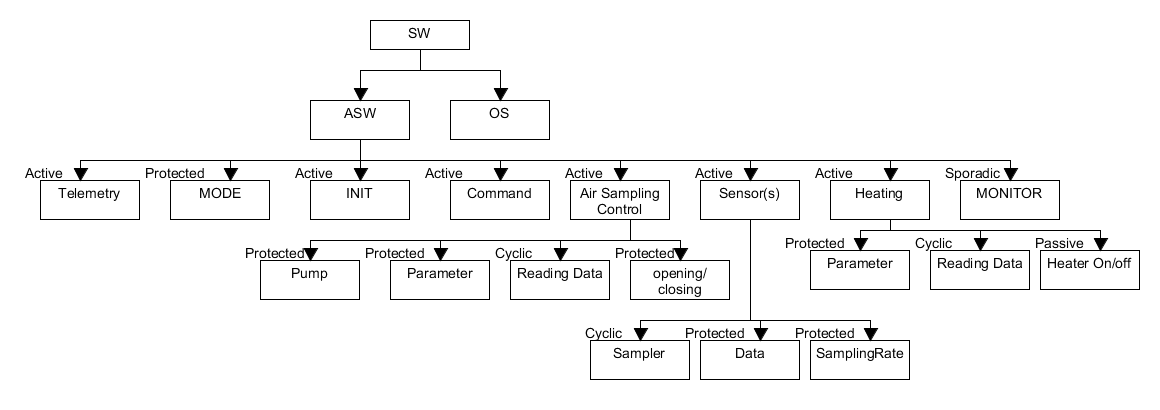
\includegraphics[width=1\linewidth]{4-experiment-design/img/sw_design.png}
    \end{align*}
    \caption{Onboard Software Design Tree.}\label{fig:obtree}
\end{figure}

The software design is produced by using object oriented approach. The functionality of the experiment has been divided into several objects and their children. The design tree is shown in Figure \ref{fig:obtree}.\\
\\
The Telemetry object is responsible to format the sensor/housekeeping data, and to transmit it. MODE is responsible for controlling the four modes of software. INIT will initialize the necessary software programs. COMMANDS reads the telecommands and execute their commands. The AIR SAMPLING CONTROL object have the four children objects. The first child is responsible for controlling the pump. The second child contains the parameters for the valves and pump. The third child reads the data from the sensors, a fourth child is responsible for manipulating the valves.\\
\\
The SENSOR object have two children objects. One for sampling the sensors and another for recording and storing the housekeeping data. The HEATER object have three children objects. One for reading the temperature sensor data, another for deciding if the heaters should be turn on/off. And the third child for turning it on/off.\\ 
\\
The MONITOR object utilizes a watchdog timer that causes an interrupt when it reaches 0, underflow. The watchdog does not get fed directly from by the end of the different tasks. Instead the tasks sets a flag, if all the flags are set the watchdog gets reset and the countdown starts from the beginning. If the watchdog times out before all the flags are set the monitor object resets the board.\\
\\
Each of the objects interacts with each others fulfilling mutually exclusive interaction. It means that any shared variables can only be accessed by one object at time. This is important considering the program is be fully automatic and to prevent unnecessary data lost. The objects interface diagrams and their sequence diagrams can be found in Appendix \ref{sec:appB} and \ref{sec:appC}.
\end{enumerate}
%\begin{figure}[H]
%    \centering
%    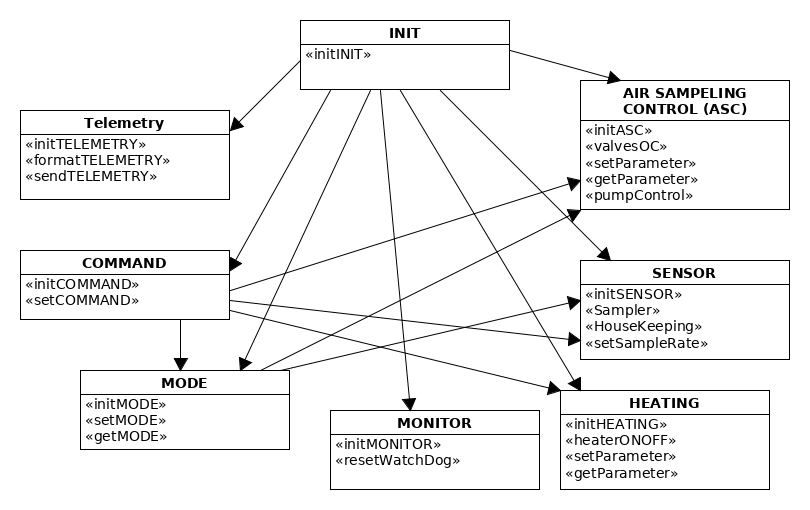
\includegraphics[width=1\textwidth]{4-experiment-design/img/hood-diagram-v1-0.png}
%    \caption{Hierarchic Object-Oriented Design of the software}
%    \label{fig:hood}
%\end{figure}
\subsubsection{Implementation}\label{sec:4.8.3}
The C/C++ programming language is used when programming the platform. Software's as PlatformIO IDE is used, other software will be used if necessary. The software is functioning autonomously using real-time operating system. FreeRTOS is chosen as the real-time operating system, which provides feature to split functionality into several mutual exclusive tasks. These tasks are \begin{itemize}
    \item The Sampler task (periodic)
    \item The Reading task (periodic)
    \item heaterTask task (periodic)
    \item telecommand task (sporadic)
\end{itemize} 
Several libraries that are used:
\begin{itemize}
    \item FreeRTOS\_ARM.h (FreeRTOS specially port for ARM microprocessor like Due)
    \item ArduinoSTL.h (allows standard C++ functionality)
    \item RTCDue.h (keeps track of the time from the software start)
    \item Necessary Arduino libraries.
    \item Sensors libraries.
\end{itemize}


\raggedbottom